\documentclass[12pt,a4paper]{article}
\usepackage[utf8]{inputenc} %polskie znaki
\usepackage[T1]{fontenc}	%polskie znaki
\usepackage{amsmath}		%matematyczne znaczki :3
\usepackage{enumerate}		%Dodatkowe opcje do funkcji enumerate
\usepackage{geometry} 		%Ustawianie marginesow
\usepackage{graphicx}		%Grafika
\usepackage{wrapfig}		%Grafika obok textu
\usepackage{float}			%Allows H in fugire
\usepackage{hyperref}		%Allows hyperlinks
%\pagestyle{empty} 			%usuwa nr strony
\usepackage{todonotes}		%Todo notatki
\usepackage{lipsum}         %Lorem text
\usepackage{ntheorem}   	% for theorem-like environments
\usepackage{mdframed}   	% for framing
\usepackage{subcaption}		% subfigure (image placing)

\newgeometry{tmargin=2cm, bmargin=2cm, lmargin=2cm, rmargin=2cm} 

\newcommand\uwaga[1]{\textcolor{orange}{#1}}
\newcommand\TODO[1]{\textcolor{red}{#1}}

\theoremstyle{break}
\theoreminframepreskip{0.5cm}
\theoremheaderfont{\bfseries}
\newmdtheoremenv[%
linecolor=white,%
innertopmargin=\topskip,
shadowsize=0,%
innertopmargin=5,%
innerbottommargin=5,%
leftmargin=10,%
rightmargin=10,%
backgroundcolor=gray!20,%
innertopmargin=0pt,%
ntheorem]{zad}{Zadanie}

\begin{document}
	
	\begin{center}
		\LARGE Zadania na lekcje 1 - podstawy algebry
	\end{center}
	\vspace{1.5cm}
	
	\begin{zad}
		Rozwiąż równania:
	\end{zad}
	\begin{enumerate}[a)] \begin{tabular}{p{7cm} p{7cm}} 
		\item $2(x-3)=3(x+5)$ & \vspace{0.25cm} 	\item$4(x+4)-2(3x-5)=8$ \\
		\item $2(x-3)-3(6+x)=6-(3+x)$ & \item $2-x<x+7$ \\
		\item $3x+5(x-3)\geq 14-(x+4)$ & \item $\frac{x-1}{2}+\frac{1}{4}(x-1)=9$ \\
		\item $\frac{1}{3}(x+3)+\frac{x}{5} - x < 4 - \frac{x-3}{15}$ & \item $\frac{2x+5}{3}-\frac{x-7}{6}$> $\frac{1}{2}$ \\
		\item $2(x-3)<\frac{2-x}{3}+\frac{3}{2}(x-5)$ & \item $\frac{1}{2}(x-3)-\frac{6+x}{3}<\frac{x}{6}$ \\
	\end{tabular} \end{enumerate}

	\begin{zad}
		Dla poniższych równań i nierówności przedstaw ich interpretacje, a następnie rozwiąż:
	\end{zad}
	\begin{enumerate}[a)] \begin{tabular}{p{7cm} p{7cm}} 
		\item $|x-3|=5$ & \vspace{0.25cm} 	\item$|x+4|<4$ \\
		\item $|x+5|=-2$ & \item $|x+6|>2\frac{1}{5}$ \\
		\item $|2x-3|=6$ & \item $-|4-x|>-2$ \\
	\end{tabular} \end{enumerate}
	
	\begin{zad}
		Rozpisz korzystając ze wzorów skróconego mnożenia:
	\end{zad}
	\begin{enumerate}[a)] \begin{tabular}{p{5cm} p{5cm} p{5cm}} 
			\item $(x+2)^2$ & \vspace{0.25cm}\item$(x-3)^2$ &\vspace{0.25cm}\item $(2x+5)^2$\\
			\item $(x+2y)^2$ & \item $(3+2x)^2$ &\item $(5x+2)^2$\\
			\item $(-x-2)^2$ & \item $(-3y+7)^2$ &\item $(-5x+3)^2$\\
			\item $(x-2y)(x+2y)$ & \item $(3x+1)(3x-1)$ &\item $(4+5x)(5x-4)$\\
			\item $(x^2-4)(x^2+4)$ & \item $(4a+7b)(7b-4a)$ &\item $(-x-2y)(2y-x)$\\
	\end{tabular} \end{enumerate}
\newpage
	\begin{zad}
		Rozpisz korzystając ze wzorów skróconego mnożenia:
	\end{zad}

		\begin{enumerate}[a)] \begin{tabular}{p{8cm} p{8cm}} 
			\item $(x+2y)^2+(x-2y)^2$ & \vspace{0.25cm}\item$(3x-4)^2-(3x+4)^2$ \\
			\item $(5x-3y)^2+(3x-5y)^2$ & \item $(x+\frac{1}{2}y)(x-\frac{1}{2}y)-(\frac{1}{2}y-x)(x+\frac{1}{2}y)$ \\
			\item $(2\sqrt{2}-8)^2-(3\sqrt{3}+2\sqrt{2})^2$ & \item $(\sqrt{5}-2\sqrt{2})(2\sqrt{2}+\sqrt{5})-(4\sqrt{3}+2\sqrt{2})^2$ \\
	\end{tabular} \end{enumerate}

	\begin{zad}
		Udowonij, że liczba
		$$(x+1)^2+(x-1)^2$$
		jest podzielna przez 2, dla każdej liczby naturalnej x.
	\end{zad}

	\begin{zad}
		Udowonij, że liczba
		$$(x+4)^2+(x-3)^2-(x+4)^2-(x-1)^2$$
		jest podzielna przez 4, dla każdej liczby naturalnej x.
	\end{zad}

	\begin{zad}
		Udowonij, że suma dwóch kolejnych parzystych liczb naturalnych jest podzielna przez 4.
	\end{zad}

	\begin{zad}
		Udowonij, że suma dwóch kolejnych nieparzystych liczb naturalnych przy dzieleniu przez 4 daje resztę 2.
	\end{zad}

	\begin{zad}
	Udowonij, liczba
	$$x^2+3x+2$$
	jest podzielna przez 2.
	\end{zad}

	\begin{zad}
		Wykaż, że dla dowolnych liczb rzeczywistych x,y prawdziwe są nierówności:
	\end{zad}
	\begin{enumerate}[a)]
		\item $x^2+2xy+3y^2\geq 0$
		\item $2x^2+25x^2\geq 10xy$
		\item $x^4y^2+2x^3y^3+x^2y^4\geq0$
		\item $\frac{3x^2}{4}+\frac{y^2}{3}-xy\geq0$
	\end{enumerate}

	\newpage

\begin{center}
	\LARGE Zbiór zadań - podstawy algebry
\end{center}
		\begin{mdframed}[%
		linecolor=white,%
		innertopmargin=\topskip,
		shadowsize=0,%
		innertopmargin=5,%
		innerbottommargin=5,%
		leftmargin=10,%
		rightmargin=10,%
		backgroundcolor=gray!20,%
		innertopmargin=0pt,]
		\vspace{0.2cm}
		\textbf{1.} Rozwiąż równania:
	\end{mdframed}

	\begin{enumerate}[a)] \begin{tabular}{p{7cm} p{7cm}} 
		\item $2(x-3)=3(x+5)$ & \vspace{0.25cm} 	\item$4(x+4)-2(3x-5)=8$ \\
		\item $2(x-3)-3(6+x)=6-(3+x)$ & \item $2-x<x+7$ \\
		\item $3x+5(x-3)\geq 14-(x+4)$ & \item $\frac{x-1}{2}+\frac{1}{4}(x-1)=9$ \\
		\item $\frac{1}{3}(x+3)+\frac{x}{5} - x < 4 - \frac{x-3}{15}$ & \item $\frac{2x+5}{3}-\frac{x-7}{6}$> $\frac{1}{2}$ \\
		\item $2(x-3)<\frac{2-x}{3}+\frac{3}{2}(x-5)$ & \item $\frac{1}{2}(x-3)-\frac{6+x}{3}<\frac{x}{6}$ \\
	\end{tabular} \end{enumerate}

			\begin{mdframed}[%
		linecolor=white,%
		innertopmargin=\topskip,
		shadowsize=0,%
		innertopmargin=5,%
		innerbottommargin=5,%
		leftmargin=10,%
		rightmargin=10,%
		backgroundcolor=gray!20,%
		innertopmargin=0pt,]
		\vspace{0.2cm}
		\textbf{2.} Rozpisz korzystając ze wzorów skróconego mnożenia:
	\end{mdframed}
	
	\begin{enumerate}[a)] \begin{tabular}{p{5cm} p{5cm} p{5cm}} 
		\item $(9-4y)^2$ & \vspace{0.25cm}\item$(x-3)^2$ &\vspace{0.25cm}\item $(2x+5)^2$\\
		\item $(4+3e)^2$ & \item $(3+2x)^2$ &\item $(5x+2)^2$\\
		\item $(a+1)^2$ & \item $(4-3a)^2$ &\item $(2b-6x)^2$\\
		\item $(a+1)^2$ & \item $(4-3a)^2$ &\item $(2b-6x)^2$\\
		\item $(-x-2)^2$ & \item $(-3y+7)^2$ &\item $(-5x+3)^2$\\
		\item $(x-2y)(x+2y)$ & \item $(3x+1)(3x-1)$ &\item $(4+5x)(5x-4)$\\
		\item $(x^2-4)(x^2+4)$ & \item $(4a+7b)(7b-4a)$ &\item $(-x-2y)(2y-x)$\\
\end{tabular} \end{enumerate}

			\begin{mdframed}[%
	linecolor=white,%
	innertopmargin=\topskip,
	shadowsize=0,%
	innertopmargin=5,%
	innerbottommargin=5,%
	leftmargin=10,%
	rightmargin=10,%
	backgroundcolor=gray!20,%
	innertopmargin=0pt,]
	\vspace{0.2cm}
	\textbf{3.} Rozpisz korzystając ze wzorów skróconego mnożenia:
\end{mdframed}

	\begin{enumerate}[a)] \begin{tabular}{p{8cm} p{8cm}} 
		\item $5y^2-3(y+1)(y-1)$ & \vspace{0.25cm}\item$(4+3y)(4-3y)-(4-y)^2$ \\
		\item $(3x+1)(3x+1)+(1+5x)(1-5x)$ & \item $(x-7)^2-(4-2x)^2$ \\
		\item $(\sqrt{2}+2)^2+(\sqrt{3}-3)^2$ & \item $(2-\sqrt{5})(2+\sqrt{5})-(2-\sqrt{5})^2$ \\
	\end{tabular} \end{enumerate}
	\newpage
				\begin{mdframed}[%
		linecolor=white,%
		innertopmargin=\topskip,
		shadowsize=0,%
		innertopmargin=5,%
		innerbottommargin=5,%
		leftmargin=10,%
		rightmargin=10,%
		backgroundcolor=gray!20,%
		innertopmargin=0pt,]
		\vspace{0.2cm}
		\textbf{4.} Usuń niewymierność z podanych wyrażeń:
	\end{mdframed}
	
	\begin{enumerate}[a)] \begin{tabular}{p{5cm} p{5cm} p{5cm}} 
			\item \Large$\frac{1}{\sqrt{2}}$ & \vspace{0.25cm}\item\Large$\frac{4}{2\sqrt{2}}$ &\vspace{0.25cm}\item \Large$\frac{6\sqrt{2}}{\sqrt{3}}$\\
			\item \Large$\frac{1}{1+\sqrt{2}}$ & \item \Large$\frac{4}{\sqrt{5}-1}$ &\item \Large$\frac{2\sqrt{6}}{\sqrt{6}+2}$\\
			\item \Large$\frac{2+\sqrt{5}}{\sqrt{5}-1}$ & \item \Large$\frac{\sqrt{2}+3}{3-\sqrt{2}}$ &\item \Large$\frac{5+\sqrt{3}}{3+\sqrt{5}}$\\
	\end{tabular} \end{enumerate}
	
					\begin{mdframed}[%
		linecolor=white,%
		innertopmargin=\topskip,
		shadowsize=0,%
		innertopmargin=5,%
		innerbottommargin=5,%
		leftmargin=10,%
		rightmargin=10,%
		backgroundcolor=gray!20,%
		innertopmargin=0pt,]
		\vspace{0.2cm}
		\textbf{4.} Poniżej przedstawiono interpretację geometryczną w postaci przedziału pewnej nierówności:
	\end{mdframed}

	\begin{figure}[h]
		\centering
		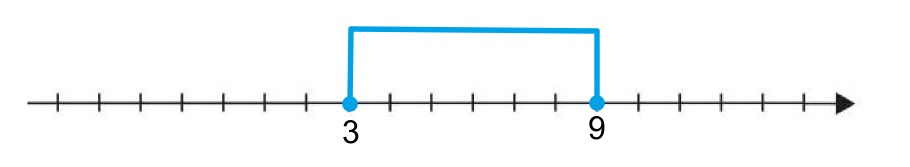
\includegraphics[scale=0.5]{z1_1.jpeg}
	\end{figure}
	
	Nierówność opisującą ten przedział można opisać za pomocą:
	
		\vspace{0.5cm}
	\begin{tabular}{p{5cm} p{5cm}}
		\textbf{A. }$|x+6|\leq3$&
		\textbf{B. }$|x-6|\leq3$\\
		\textbf{C. }$|x+6|\geq3$&
		\textbf{D. }$|x-6|\geq3$\\
	\end{tabular}

					\begin{mdframed}[%
	linecolor=white,%
	innertopmargin=\topskip,
	shadowsize=0,%
	innertopmargin=5,%
	innerbottommargin=5,%
	leftmargin=10,%
	rightmargin=10,%
	backgroundcolor=gray!20,%
	innertopmargin=0pt,]
	\vspace{0.2cm}
	\textbf{5.} Nierówność $|x-2|>4$ można przedstawić za pomocą przedziału:
\end{mdframed}

\begin{figure}[h]
	\centering
	\begin{subfigure}[b]{0.45\textwidth}
		\Large \textbf{A}
		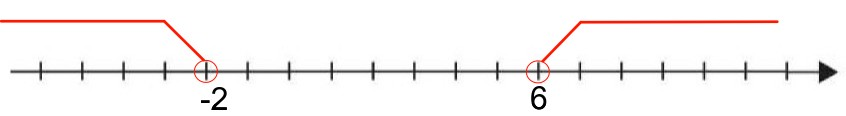
\includegraphics[width=\textwidth]{z1_2_1.jpeg}
		
	\end{subfigure}$\quad$
	\begin{subfigure}[b]{0.45\textwidth}
		\Large \textbf{B}
	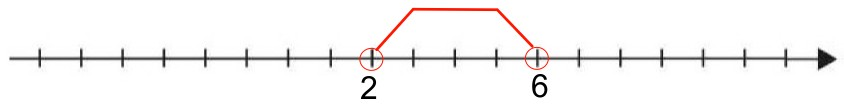
\includegraphics[width=\textwidth]{z1_2_2.jpeg}
	
\end{subfigure}
\end{figure}
\begin{figure}[h]
	\centering
	\begin{subfigure}[b]{0.45\textwidth}
		\Large \textbf{C}
		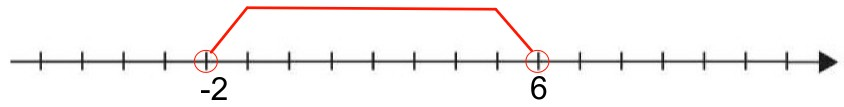
\includegraphics[width=\textwidth]{z1_2_3.jpeg}
		
	\end{subfigure}$\quad$
	\begin{subfigure}[b]{0.45\textwidth}
		\Large \textbf{D}
		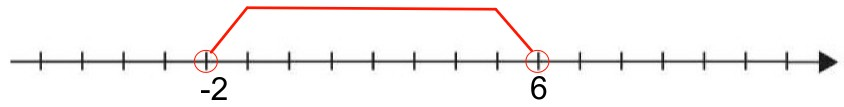
\includegraphics[width=\textwidth]{z1_2_3.jpeg}
	\end{subfigure}
\end{figure}

					\begin{mdframed}[%
	linecolor=white,%
	innertopmargin=\topskip,
	shadowsize=0,%
	innertopmargin=5,%
	innerbottommargin=5,%
	leftmargin=10,%
	rightmargin=10,%
	backgroundcolor=gray!20,%
	innertopmargin=0pt,]
	\vspace{0.2cm}
	\textbf{6.} Udowodnij, że liczba $$(2x+1)^2-(x+1)^2+x$$ jest podzielna przez 6.
\end{mdframed}

					\begin{mdframed}[%
	linecolor=white,%
	innertopmargin=\topskip,
	shadowsize=0,%
	innertopmargin=5,%
	innerbottommargin=5,%
	leftmargin=10,%
	rightmargin=10,%
	backgroundcolor=gray!20,%
	innertopmargin=0pt,]
	\vspace{0.2cm}
	\textbf{7.} Udowodnij, że liczba $$5x^3-5x$$ jest podzielna przez 30.
\end{mdframed}
	
\end{document}